\documentclass{article}\usepackage[]{graphicx}\usepackage[]{color}
%% maxwidth is the original width if it is less than linewidth
%% otherwise use linewidth (to make sure the graphics do not exceed the margin)
\makeatletter
\def\maxwidth{ %
  \ifdim\Gin@nat@width>\linewidth
    \linewidth
  \else
    \Gin@nat@width
  \fi
}
\makeatother

\definecolor{fgcolor}{rgb}{0.345, 0.345, 0.345}
\newcommand{\hlnum}[1]{\textcolor[rgb]{0.686,0.059,0.569}{#1}}%
\newcommand{\hlstr}[1]{\textcolor[rgb]{0.192,0.494,0.8}{#1}}%
\newcommand{\hlcom}[1]{\textcolor[rgb]{0.678,0.584,0.686}{\textit{#1}}}%
\newcommand{\hlopt}[1]{\textcolor[rgb]{0,0,0}{#1}}%
\newcommand{\hlstd}[1]{\textcolor[rgb]{0.345,0.345,0.345}{#1}}%
\newcommand{\hlkwa}[1]{\textcolor[rgb]{0.161,0.373,0.58}{\textbf{#1}}}%
\newcommand{\hlkwb}[1]{\textcolor[rgb]{0.69,0.353,0.396}{#1}}%
\newcommand{\hlkwc}[1]{\textcolor[rgb]{0.333,0.667,0.333}{#1}}%
\newcommand{\hlkwd}[1]{\textcolor[rgb]{0.737,0.353,0.396}{\textbf{#1}}}%

\usepackage{framed}
\makeatletter
\newenvironment{kframe}{%
 \def\at@end@of@kframe{}%
 \ifinner\ifhmode%
  \def\at@end@of@kframe{\end{minipage}}%
  \begin{minipage}{\columnwidth}%
 \fi\fi%
 \def\FrameCommand##1{\hskip\@totalleftmargin \hskip-\fboxsep
 \colorbox{shadecolor}{##1}\hskip-\fboxsep
     % There is no \\@totalrightmargin, so:
     \hskip-\linewidth \hskip-\@totalleftmargin \hskip\columnwidth}%
 \MakeFramed {\advance\hsize-\width
   \@totalleftmargin\z@ \linewidth\hsize
   \@setminipage}}%
 {\par\unskip\endMakeFramed%
 \at@end@of@kframe}
\makeatother

\definecolor{shadecolor}{rgb}{.97, .97, .97}
\definecolor{messagecolor}{rgb}{0, 0, 0}
\definecolor{warningcolor}{rgb}{1, 0, 1}
\definecolor{errorcolor}{rgb}{1, 0, 0}
\newenvironment{knitrout}{}{} % an empty environment to be redefined in TeX

\usepackage{alltt}
\usepackage[latin1]{inputenc} % utilice "latin1" si 
\usepackage{multienum}
\usepackage{multicol}
\usepackage{tikz}
\IfFileExists{upquote.sty}{\usepackage{upquote}}{}
\begin{document}

Este es el analisis para una serie real
Visualizacion de la serie
\begin{knitrout}
\definecolor{shadecolor}{rgb}{0.969, 0.969, 0.969}\color{fgcolor}\begin{kframe}
\begin{alltt}
\hlkwd{library}\hlstd{(}\hlstr{"TSA"}\hlstd{)}
\end{alltt}


{\ttfamily\noindent\color{warningcolor}{\#\# Warning: package 'TSA' was built under R version 3.2.2}}

{\ttfamily\noindent\itshape\color{messagecolor}{\#\# Loading required package: leaps}}

{\ttfamily\noindent\color{warningcolor}{\#\# Warning: package 'leaps' was built under R version 3.2.2}}

{\ttfamily\noindent\itshape\color{messagecolor}{\#\# Loading required package: locfit}}

{\ttfamily\noindent\color{warningcolor}{\#\# Warning: package 'locfit' was built under R version 3.2.2}}

{\ttfamily\noindent\itshape\color{messagecolor}{\#\# locfit 1.5-9.1 	 2013-03-22\\\#\# Loading required package: mgcv\\\#\# Loading required package: nlme\\\#\# This is mgcv 1.8-6. For overview type 'help("{}mgcv-package"{})'.\\\#\# Loading required package: tseries}}

{\ttfamily\noindent\color{warningcolor}{\#\# Warning: package 'tseries' was built under R version 3.2.2}}

{\ttfamily\noindent\itshape\color{messagecolor}{\#\# \\\#\# Attaching package: 'TSA'\\\#\# \\\#\# The following objects are masked from 'package:stats':\\\#\# \\\#\#\ \ \ \  acf, arima\\\#\# \\\#\# The following object is masked from 'package:utils':\\\#\# \\\#\#\ \ \ \  tar}}\begin{alltt}
\hlkwd{library}\hlstd{(}\hlstr{"leaps"}\hlstd{)}
\hlkwd{library}\hlstd{(}\hlstr{"locfit"}\hlstd{)}
\hlkwd{library}\hlstd{(}\hlstr{"tseries"}\hlstd{)}
\hlstd{basemz}\hlkwb{=}\hlkwd{read.table}\hlstd{(}\hlstr{"maiz.txt"}\hlstd{,}\hlkwc{header}\hlstd{=}\hlnum{TRUE}\hlstd{)}
\hlstd{basemz}
\end{alltt}
\begin{verbatim}
##    maiz
## 1  0.18
## 2  0.17
## 3  0.17
## 4  0.17
## 5  0.17
## 6  0.18
## 7  0.18
## 8  0.19
## 9  0.21
## 10 0.20
## 11 0.19
## 12 0.19
## 13 0.21
## 14 0.23
## 15 0.24
## 16 0.27
## 17 0.30
## 18 0.38
## 19 0.36
## 20 0.37
## 21 0.29
## 22 0.25
## 23 0.23
## 24 0.23
## 25 0.22
## 26 0.23
## 27 0.23
## 28 0.23
## 29 0.23
## 30 0.22
## 31 0.22
## 32 0.22
## 33 0.22
## 34 0.20
## 35 0.19
## 36 0.20
## 37 0.19
## 38 0.18
## 39 0.19
## 40 0.20
## 41 0.19
## 42 0.19
## 43 0.20
## 44 0.20
## 45 0.20
## 46 0.19
## 47 0.19
## 48 0.18
## 49 0.18
## 50 0.18
## 51 0.19
## 52 0.19
## 53 0.18
## 54 0.20
## 55 0.22
## 56 0.26
## 57 0.24
## 58 0.23
## 59 0.22
## 60 0.22
## 61 0.24
## 62 0.24
## 63 0.25
## 64 0.25
## 65 0.24
## 66 0.24
## 67 0.27
## 68 0.25
## 69 0.25
## 70 0.24
\end{verbatim}
\begin{alltt}
\hlstd{mz}\hlkwb{=}\hlkwd{ts}\hlstd{(basemz}\hlopt{$}\hlstd{maiz,}\hlkwc{start}\hlstd{=}\hlkwd{c}\hlstd{(}\hlnum{2010}\hlstd{,}\hlnum{1}\hlstd{),}\hlkwc{end}\hlstd{=}\hlkwd{c}\hlstd{(}\hlnum{2015}\hlstd{,}\hlnum{10}\hlstd{),}\hlkwc{frequency} \hlstd{=} \hlnum{12}\hlstd{,}\hlkwc{names}\hlstd{=}\hlstr{"Precio del maíz"}\hlstd{)}
\hlkwd{plot}\hlstd{(mz,}\hlkwc{type}\hlstd{=}\hlstr{"o"}\hlstd{,} \hlkwc{xlab}\hlstd{=}\hlstr{"Año"}\hlstd{,} \hlkwc{ylab} \hlstd{=} \hlstr{"Precio del maíz"}\hlstd{,}\hlkwc{main}\hlstd{=}\hlstr{"Gráfico del precio del maíz de Enero/2010-Octubre/2015"}\hlstd{)}
\end{alltt}
\end{kframe}
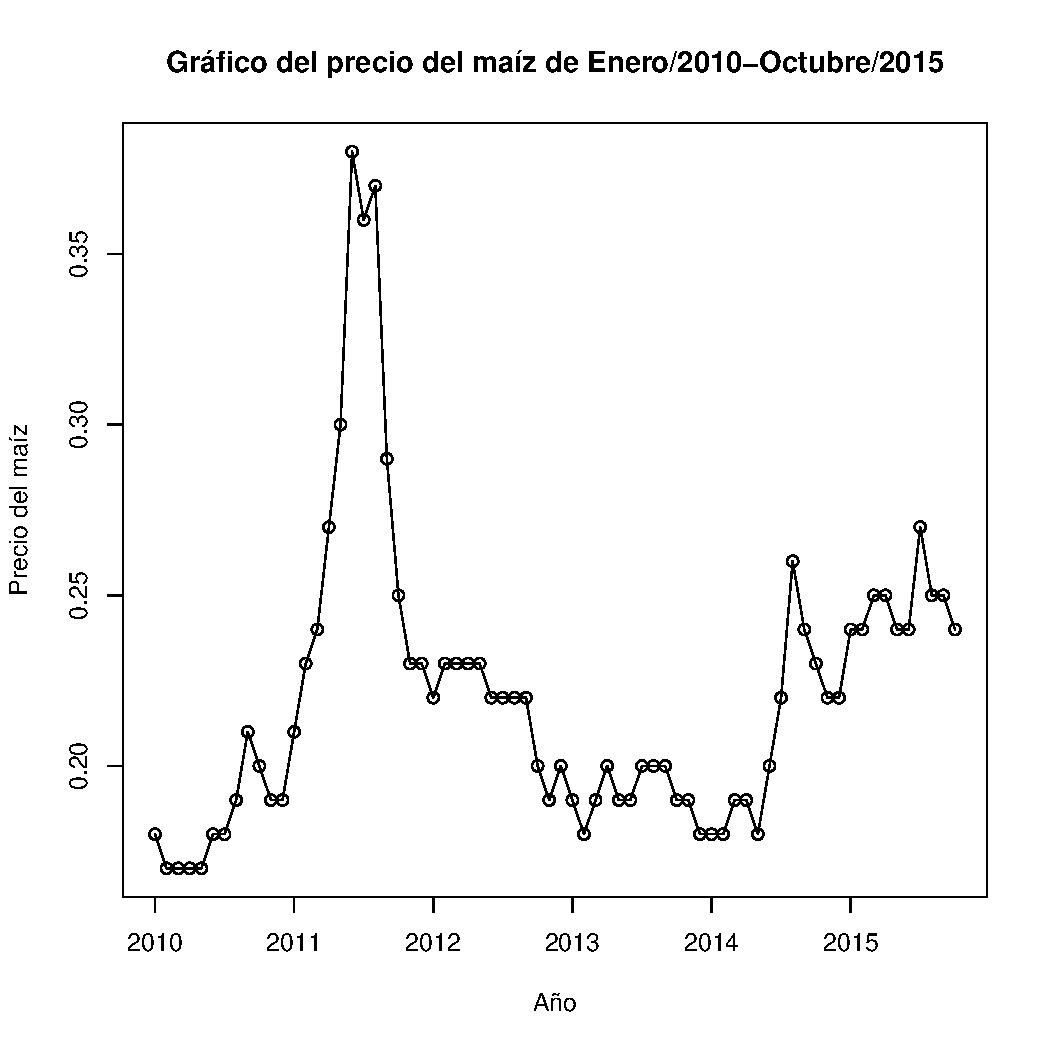
\includegraphics[width=\maxwidth]{figure/unnamed-chunk-1-1} 

\end{knitrout}

Analisis de estacionariedad


De los resultados anterires se concluye que solomente se hara una diferencia a las serie

\begin{knitrout}
\definecolor{shadecolor}{rgb}{0.969, 0.969, 0.969}\color{fgcolor}\begin{kframe}
\begin{alltt}
\hlkwd{library}\hlstd{(}\hlstr{"TSA"}\hlstd{)}
\hlkwd{library}\hlstd{(}\hlstr{"leaps"}\hlstd{)}
\hlkwd{library}\hlstd{(}\hlstr{"locfit"}\hlstd{)}
\hlkwd{library}\hlstd{(}\hlstr{"tseries"}\hlstd{)}
\hlkwd{acf}\hlstd{(}\hlkwd{diff}\hlstd{(mz))}
\end{alltt}
\end{kframe}
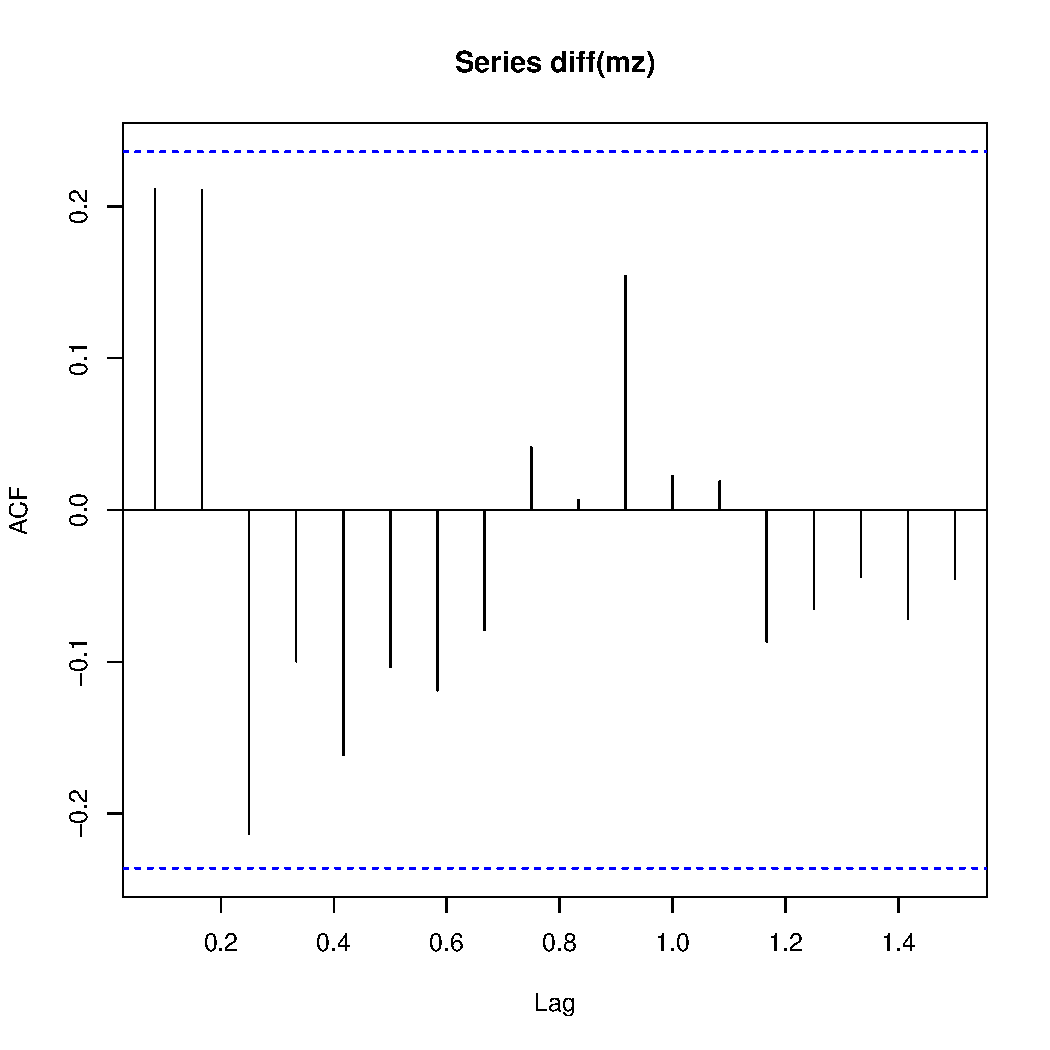
\includegraphics[width=\maxwidth]{figure/unnamed-chunk-2-1} 
\begin{kframe}\begin{alltt}
\hlkwd{pacf}\hlstd{(}\hlkwd{diff}\hlstd{(mz))}
\end{alltt}
\end{kframe}
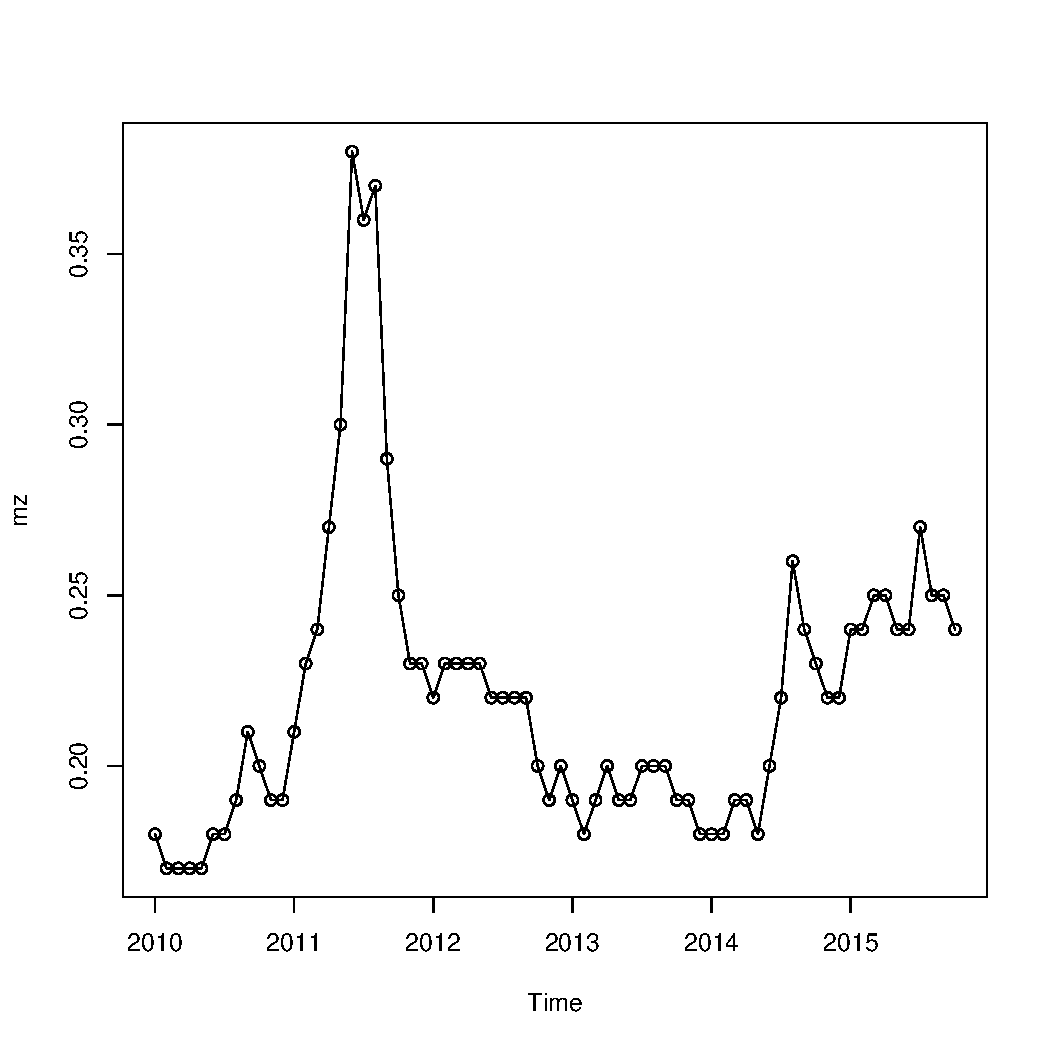
\includegraphics[width=\maxwidth]{figure/unnamed-chunk-2-2} 
\begin{kframe}\begin{alltt}
\hlkwd{eacf}\hlstd{(}\hlkwd{diff}\hlstd{(mz))}
\end{alltt}
\begin{verbatim}
## AR/MA
##   0 1 2 3 4 5 6 7 8 9 10 11 12 13
## 0 o o o o o o o o o o o  o  o  o 
## 1 x o x o o o o o o o o  o  o  o 
## 2 x x x o o o o o o o o  o  o  o 
## 3 o o o o o o o o o o o  o  o  o 
## 4 x o o o o o o o o o o  o  o  o 
## 5 o o o o o o o o o o o  o  o  o 
## 6 x o x o o o o o o o o  o  o  o 
## 7 x o o o o o o o o o o  o  o  o
\end{verbatim}
\begin{alltt}
\hlstd{cua}\hlkwb{=}\hlkwd{armasubsets}\hlstd{(}\hlkwc{y}\hlstd{=}\hlkwd{diff}\hlstd{(mz),}\hlkwc{nar}\hlstd{=}\hlnum{7}\hlstd{,}\hlkwc{nma}\hlstd{=}\hlnum{7}\hlstd{,}
                \hlkwc{y.name}\hlstd{=}\hlstr{'test'}\hlstd{,} \hlkwc{ar.method}\hlstd{=}\hlstr{'ols'}\hlstd{)}
\hlkwd{plot}\hlstd{(cua)}
\end{alltt}
\end{kframe}
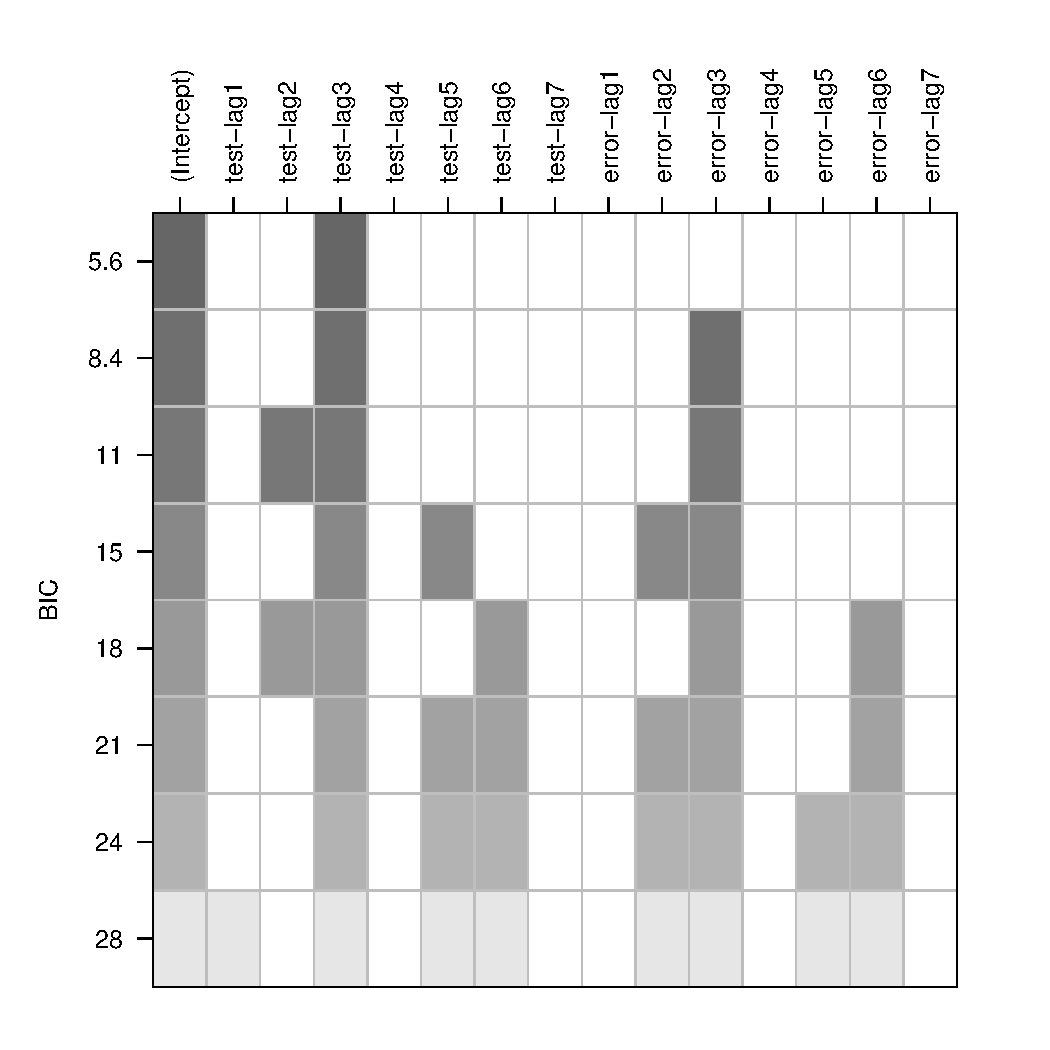
\includegraphics[width=\maxwidth]{figure/unnamed-chunk-2-3} 

\end{knitrout}

Modelos que podrian a probar:
ARI(3,1)

ARIMA(1,1,3)

ARIMA(3,1,3)

estimacion de parametros
Se toma el ARI(3) para probarlo
\begin{knitrout}
\definecolor{shadecolor}{rgb}{0.969, 0.969, 0.969}\color{fgcolor}\begin{kframe}
\begin{alltt}
\hlkwd{library}\hlstd{(}\hlstr{"TSA"}\hlstd{)}
\hlkwd{library}\hlstd{(}\hlstr{"leaps"}\hlstd{)}
\hlkwd{library}\hlstd{(}\hlstr{"locfit"}\hlstd{)}
\hlkwd{library}\hlstd{(}\hlstr{"tseries"}\hlstd{)}
\hlkwd{arima}\hlstd{(}\hlkwd{diff}\hlstd{(mz),} \hlkwc{order}\hlstd{=}\hlkwd{c}\hlstd{(}\hlnum{3}\hlstd{,}\hlnum{0}\hlstd{,}\hlnum{0}\hlstd{),}\hlkwc{method}\hlstd{=}\hlstr{'ML'}\hlstd{)}
\end{alltt}
\begin{verbatim}
## 
## Call:
## arima(x = diff(mz), order = c(3, 0, 0), method = "ML")
## 
## Coefficients:
##          ar1     ar2      ar3  intercept
##       0.2249  0.2246  -0.3026     0.0009
## s.e.  0.1133  0.1128   0.1129     0.0025
## 
## sigma^2 estimated as 0.000312:  log likelihood = 180.4,  aic = -352.81
\end{verbatim}
\end{kframe}
\end{knitrout}

Validacion del modelo

\begin{knitrout}
\definecolor{shadecolor}{rgb}{0.969, 0.969, 0.969}\color{fgcolor}\begin{kframe}
\begin{alltt}
\hlstd{m1.maiz}\hlkwb{=}\hlkwd{arima}\hlstd{(}\hlkwd{diff}\hlstd{(mz),}\hlkwc{order}\hlstd{=}\hlkwd{c}\hlstd{(}\hlnum{3}\hlstd{,}\hlnum{0}\hlstd{,}\hlnum{0}\hlstd{),} \hlkwc{method}\hlstd{=}\hlstr{'ML'}\hlstd{); m1.maiz}
\end{alltt}
\begin{verbatim}
## 
## Call:
## arima(x = diff(mz), order = c(3, 0, 0), method = "ML")
## 
## Coefficients:
##          ar1     ar2      ar3  intercept
##       0.2249  0.2246  -0.3026     0.0009
## s.e.  0.1133  0.1128   0.1129     0.0025
## 
## sigma^2 estimated as 0.000312:  log likelihood = 180.4,  aic = -352.81
\end{verbatim}
\begin{alltt}
\hlkwd{plot}\hlstd{(}\hlkwd{rstandard}\hlstd{(m1.maiz),}\hlkwc{ylab} \hlstd{=}\hlstr{'Standardized Residuals'}\hlstd{,}
       \hlkwc{type}\hlstd{=}\hlstr{'o'}\hlstd{);} \hlkwd{abline}\hlstd{(}\hlkwc{h}\hlstd{=}\hlnum{0}\hlstd{)}
\end{alltt}
\end{kframe}
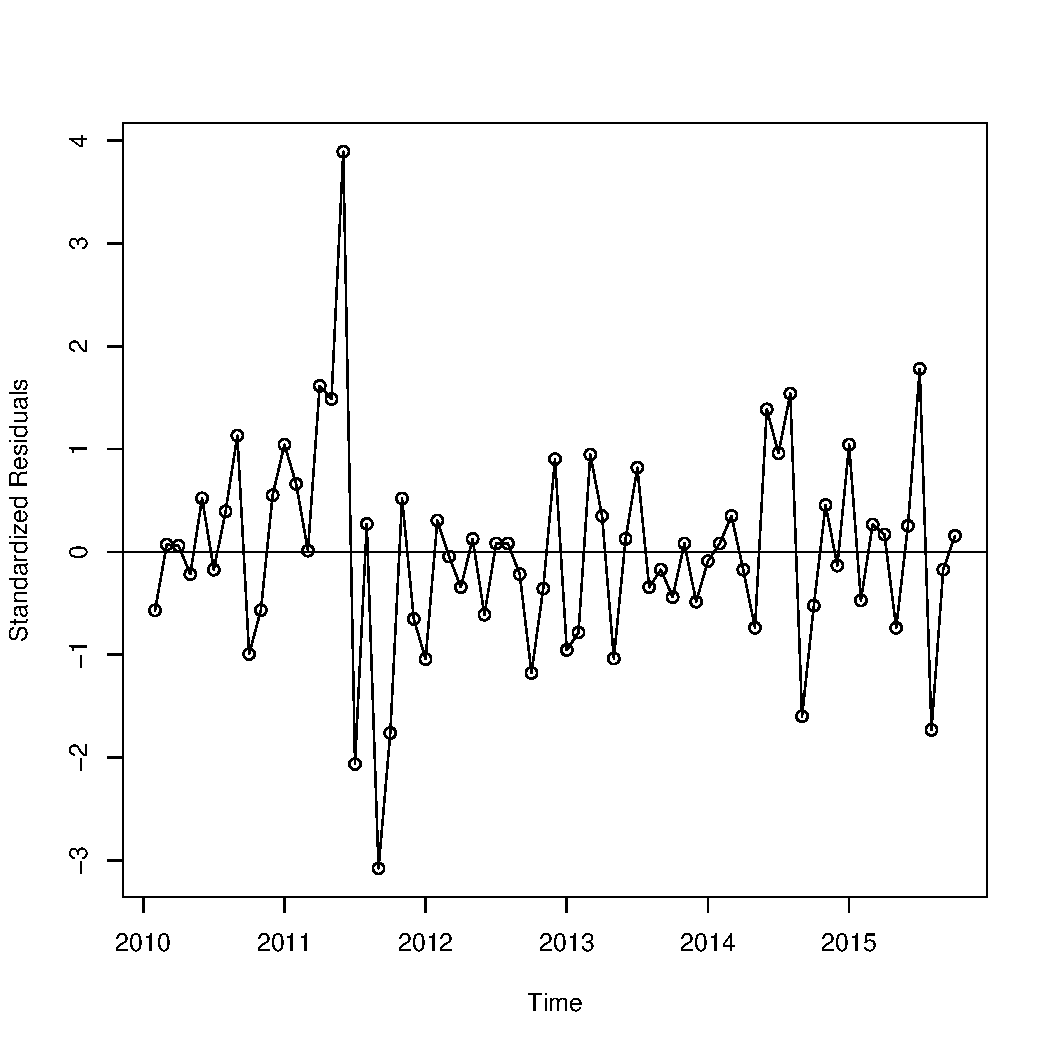
\includegraphics[width=\maxwidth]{figure/unnamed-chunk-4-1} 
\begin{kframe}\begin{alltt}
\hlkwd{qqnorm}\hlstd{(}\hlkwd{residuals}\hlstd{(m1.maiz));} \hlkwd{qqline}\hlstd{(}\hlkwd{residuals}\hlstd{(m1.maiz))}
\end{alltt}
\end{kframe}
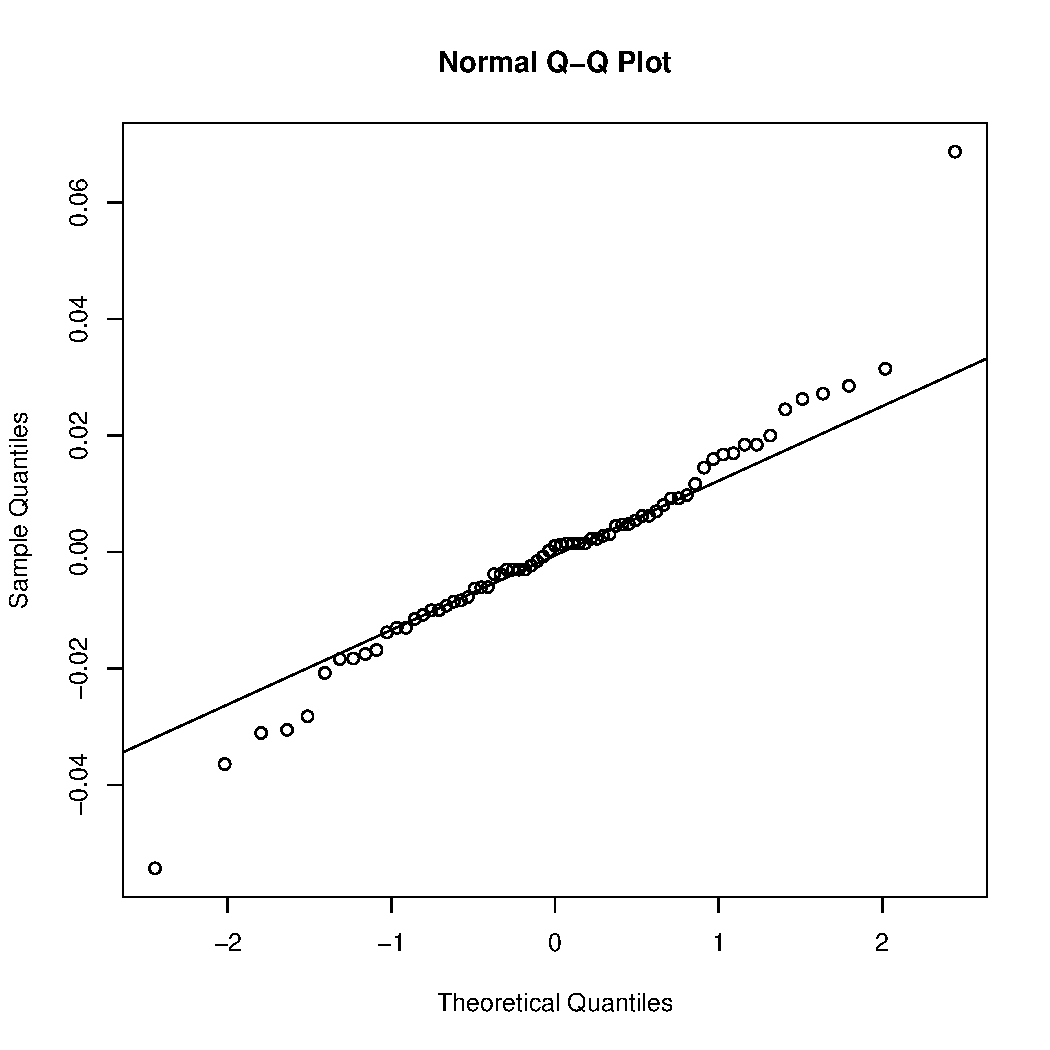
\includegraphics[width=\maxwidth]{figure/unnamed-chunk-4-2} 
\begin{kframe}\begin{alltt}
\hlkwd{acf}\hlstd{(}\hlkwd{residuals}\hlstd{(m1.maiz))}
\end{alltt}
\end{kframe}
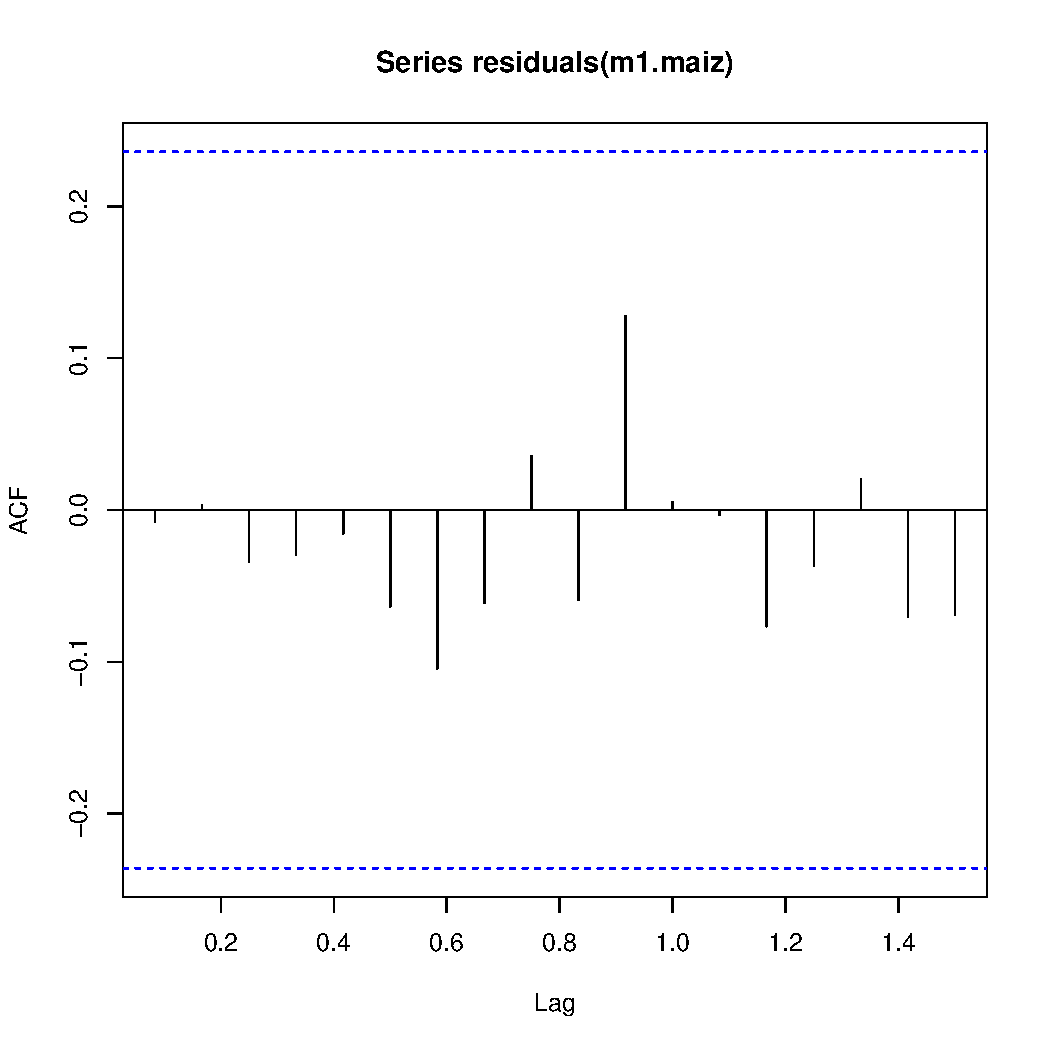
\includegraphics[width=\maxwidth]{figure/unnamed-chunk-4-3} 
\begin{kframe}\begin{alltt}
\hlkwd{tsdiag}\hlstd{(m1.maiz,}\hlkwc{gof}\hlstd{=}\hlnum{15}\hlstd{,}\hlkwc{omit.initial}\hlstd{=F)}
\end{alltt}
\end{kframe}
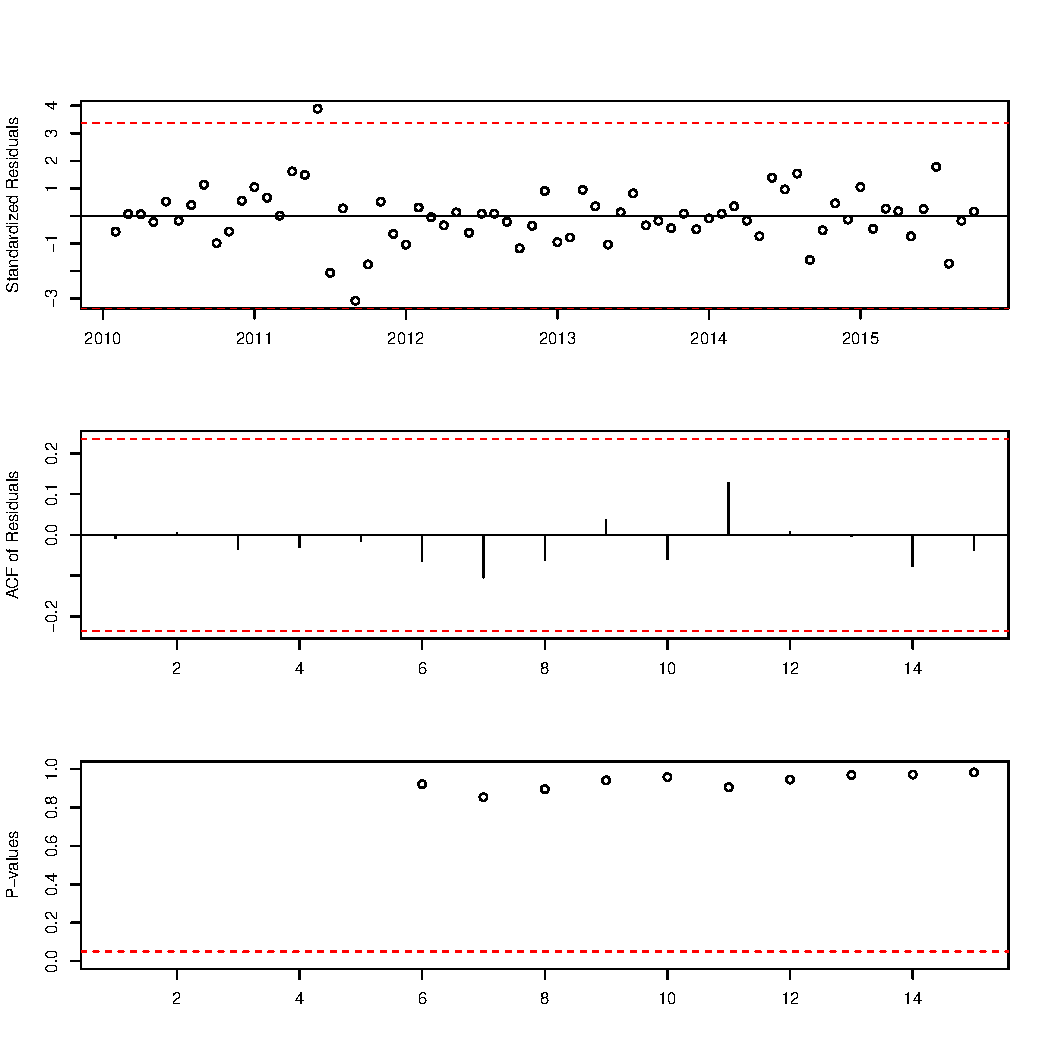
\includegraphics[width=\maxwidth]{figure/unnamed-chunk-4-4} 

\end{knitrout}

Pues sin ser tan esctrictos el modelo se validara





\end{document}
